\documentclass[11pt,a4paper]{article}

\usepackage[margin=2.5cm]{geometry}
\usepackage{graphicx}
\usepackage{hyperref}
\hypersetup{
    colorlinks=true,
    linkcolor=black,
    urlcolor=blue,
    citecolor=black,
    pdfborder={0 0 0}
}
\usepackage{amsmath}
\usepackage{booktabs}
\usepackage{enumitem}
\usepackage{float}

\begin{document}

% ----------------------------- Title page ----------------------------------
\begin{center}
    \vspace*{2cm}

    {\Huge\bfseries Project Report}

    \vspace{1.5cm}

    
\includegraphics[width=10cm]{assets/oth.png}

    \vspace{1.5cm}

    {\Large\bfseries ``Segmentation with CNNs and Transformers''}

    \vspace{2cm}

    {\small\bfseries Student}

    \vspace{0.25cm}

    {\Large\bfseries Azizjon Eshpulatov}

    \vspace{1cm}

    {\small\bfseries Professor}

    \vspace{0.25cm}

    {\Large\bfseries Prof. Dr. phil. Tatyana Ivanovska}

    \vspace{2cm}

    \begin{center}
      {\small Ostbayerische Technische Hochschule Amberg-Weiden}\\
      {\small Department of Electrical Engineering, Media and Computer Science}
    \end{center}

    \vfill
    {\large\today}
\end{center}

\title{Segmentation with CNNs and Transformers}
\author{Student: Azizjon Eshpulatov}

\newpage

\begin{center}

{\Large\bfseries ``Segmentation with CNNs and Transformers:\\
    A Controlled Comparison of U-Net and SegFormer''}

    \vspace{0.5cm}

\end{center}

\tableofcontents
\newpage

% ----------------------------- Abstract ------------------------------------
\begin{abstract}
This project presents a controlled comparison of a convolutional and a
transformer-based architecture for semantic segmentation, how each model 
combines information across the image --- local convolution versus global 
self-attention --- while holding the data, training pipeline, parameter count,
and pretraining as constant as possible. A U-Net with a ResNet-34 encoder
($\sim$24M parameters) and SegFormer with a MiT-B2 encoder ($\sim$27M
parameters) are trained on the CamVid driving-scene dataset under an identical
regime and compared along several axes: accuracy, data efficiency, robustness
to input corruptions, boundary quality, and cross-dataset generalization.
Averaged over three seeds, SegFormer outperforms U-Net
($0.798 \pm 0.002$ versus $0.765 \pm 0.007$ mean IoU), with the advantage
on thin and context-dependent classes. SegFormer is also more
data-efficient, matching U-Net's full-data accuracy using only 25\% of the
training images, substantially more robust to corruption (66.5\% versus 54.3\%
mIoU retained at maximum severity), and generalizes markedly better to an
unseen dataset: transferred zero-shot to Cityscapes the accuracy gap widens to
$+0.128$ mIoU, more than three times the in-domain gap. Across every axis the
transformer's advantage grows with the difficulty of the condition,
illustrating how the inductive biases of the two architecture families
performs on a small, class-imbalanced benchmark.
\end{abstract}

% ----------------------------- Introduction --------------------------------
\section{Introduction}

Semantic segmentation assigns a class label to every pixel of an image and is
a core task for scene understanding in applications such as autonomous driving.
For most of the past decade the dominant architectures were fully
convolutional, exemplified by the encoder--decoder U-Net and the
dilated-convolution DeepLab family. More recently, transformer-based models
that replace convolution with self-attention have matched or exceeded
convolutional networks, with SegFormer a prominent efficient example.

The two families embody opposite inductive biases. Convolution is \emph{local}
and translation-equivariant: information is aggregated within a small kernel,
and the receptive field grows only gradually with depth. Self-attention is
\emph{global} from the first layer: every position can attend to every other,
at the cost of weaker built-in spatial priors. These biases predict different
behaviour, yet head-to-head numbers in the literature often confound the
mechanism with differences in model size, pretraining data, or training recipe.

This project asks a deliberately narrow question: holding everything else
fixed, how does replacing convolution with self-attention affect segmentation
behaviour? U-Net (ResNet-34) is compared against SegFormer (MiT-B2), matched in
parameter count and ImageNet pretraining and trained with an identical
pipeline, along several axes: accuracy (overall and per class), data efficiency
(training on 25\%, 50\% and 100\% of the data), robustness to test-time image
corruptions, boundary quality, and cross-dataset generalization to Cityscapes.
The central finding is a consistent transformer advantage whose magnitude
tracks how much global context a class or condition requires.

% ----------------------------- Methodology ---------------------------------
\section{Methodology}

\subsection{Dataset}

CamVid is a road-scene dataset of $367$ training, $101$ validation and $233$
test images at $360\times480$, labelled with 11 semantic classes plus a void
class that is ignored in training and evaluation. The class distribution is
highly imbalanced: \texttt{road}, \texttt{building} and \texttt{sky} together
account for roughly 72\% of all pixels, while \texttt{bicyclist},
\texttt{pedestrian}, \texttt{sign\_symbol} and \texttt{pole} occupy under 1.2\%
each. This imbalance makes mean Intersection-over-Union (mIoU), which weights
all classes equally, the appropriate headline metric, and pixel accuracy
misleading.

\subsection{Models}

The cleanest representative of each family is deliberately selected. The
\textbf{CNN} is a U-Net with a ResNet-34 encoder ($\sim$24M parameters). The
\textbf{Transformer} is SegFormer with a MiT-B2 encoder ($\sim$27M parameters).
Both use ImageNet-pretrained encoders and are hierarchical multi-scale models
of comparable size, so that observed differences are attributable to the
feature-mixing mechanism rather than to capacity, pretraining data, or
architectural topology. SegFormer natively predicts logits at one-quarter
resolution; these are bilinearly upsampled to full resolution so that loss and
metrics are computed identically for both models.

\subsection{Training Protocol}

To keep the comparison fair, both models share one pipeline: input padded to
$384\times480$ (divisible by 32; padded pixels are labelled void), identical
augmentations (horizontal flip, brightness/contrast jitter), a combined
cross-entropy plus Dice loss, and median-frequency class weighting on the
cross-entropy term to counter imbalance. Both train for 120 epochs with AdamW,
a polynomial learning-rate schedule, and automatic mixed precision on a single
8\,GB GPU. The one intentional asymmetry is the learning rate, tuned per model
on the validation set ($3\times10^{-4}$ for U-Net, $1\times10^{-4}$ for
SegFormer); forcing an identical learning rate would handicap one architecture
and would be \emph{less} fair, not more. For the data-efficiency study, fixed
nested 25\% and 50\% subsets of the training set are drawn with a fixed seed and
used identically by both models. A 200-epoch run confirmed that both models
converge by 120 epochs (U-Net $+0.0003$, SegFormer $+0.006$ mIoU), so the
comparison is not an artifact of training length.

\subsection{Evaluation}

Per-class IoU and mIoU are reported with the void class excluded. Headline runs
are repeated over three seeds and reported as mean\,$\pm$\,standard deviation.
The test split was held out and used only once, after all tuning was frozen.
Robustness is measured by applying four corruptions (Gaussian noise, motion
blur, fog, brightness) at five severities to the evaluation images and
re-measuring mIoU, without retraining. Boundary quality is measured with
Boundary IoU, which restricts the IoU computation to a 3-pixel band around
object boundaries. Cross-dataset generalization is measured by evaluating the
CamVid-trained models on the Cityscapes validation set, with Cityscapes labels
remapped onto the CamVid class set.

% ----------------------------- Implementation ------------------------------
\section{Implementation}

\subsection{Code Structure}

The project is organized into a shared data and training core plus a set of
evaluation and analysis scripts. A single training script trains both models;
only a command-line flag and the learning rate differ, which is what keeps the
comparison fair. Table~\ref{tab:structure} lists the main components.

\begin{table}[H]
\centering
\begin{tabular}{ll}
\toprule
Path & Description \\
\midrule
\texttt{src/dataset.py}        & CamVid dataset, transforms, palette, class constants. \\
\texttt{src/class\_stats.py}   & Per-class pixel statistics and loss weights. \\
\texttt{src/make\_subsets.py}  & Fixed nested 25/50/100\% training subsets. \\
\texttt{src/losses.py}         & Combined class-weighted CE + Dice loss. \\
\texttt{src/metrics.py}        & Per-class IoU, mIoU, pixel accuracy. \\
\texttt{src/models.py}         & Model factory for U-Net and SegFormer. \\
\texttt{src/train.py}          & Shared training script for both models. \\
\texttt{src/evaluate.py}       & Per-run evaluation and prediction grids. \\
\texttt{src/aggregate\_results.py} & Summary tables and data-efficiency plot. \\
\texttt{src/compare\_models.py}    & Side-by-side qualitative comparison. \\
\texttt{src/robustness.py}     & Corruption robustness evaluation. \\
\texttt{src/boundary\_iou.py}  & Boundary-IoU edge-quality metric. \\
\texttt{src/tta\_evaluate.py}  & Test-time augmentation evaluation. \\
\texttt{src/cityscapes\_eval.py} & Zero-shot cross-dataset evaluation. \\
\bottomrule
\end{tabular}
\caption{Main components of the project.}
\label{tab:structure}
\end{table}

\subsection{Training Core}

The data pipeline (\texttt{dataset.py}) loads CamVid images and masks, applies
the shared augmentations, and pads to a network-friendly resolution while
labelling padded pixels void. The loss (\texttt{losses.py}) combines a
class-weighted cross-entropy term with a Dice term, both ignoring the void
class; the class weights are the median-frequency weights computed in
\texttt{class\_stats.py}, which counter the severe imbalance so that rare
classes such as \texttt{bicyclist} are not ignored. The model factory
(\texttt{models.py}) exposes both architectures behind one interface that
returns full-resolution logits, so the training loop, loss and metrics are
byte-for-byte identical for the two models.

\subsection{Shared Training Script}

A single script (\texttt{train.py}) trains both models. It supports
mixed-precision training, a polynomial learning-rate schedule, checkpointing of
the best and last models by validation mIoU, and per-epoch CSV logging. A small
overfit mode (training on ten images) is used as a sanity check that the whole
pipeline learns before committing to long runs. The data-efficiency subsets are
passed via a command-line flag so that both models train on identical image
lists at each data fraction.

\subsection{Evaluation and Analysis}

Evaluation (\texttt{evaluate.py}) loads a checkpoint, computes per-class IoU on
a chosen split, and renders prediction grids. Aggregation
(\texttt{aggregate\_results.py}) collects all runs into summary tables and the
data-efficiency plot. Qualitative comparison (\texttt{compare\_models.py})
renders the two models side by side on the frames where they disagree most.
The remaining scripts each implement one analysis axis: corruption robustness
(\texttt{robustness.py}), boundary quality (\texttt{boundary\_iou.py}),
test-time augmentation (\texttt{tta\_evaluate.py}), and cross-dataset
generalization (\texttt{cityscapes\_eval.py}).

% ----------------------------- Results -------------------------------------
\section{Evaluation and Results}

\subsection{Accuracy}

Table~\ref{tab:headline} reports the head-to-head comparison at full data.
SegFormer attains a mean IoU of $0.798\pm0.002$ against U-Net's
$0.765\pm0.007$ over three seeds. The $0.033$ gap exceeds six times the pooled
run-to-run standard deviation and the two models' result ranges do not overlap,
so the advantage is statistically robust; SegFormer is also the more
\emph{stable} model, with roughly one-quarter the seed variance.

\begin{table}[H]
\centering
\begin{tabular}{lccc}
\toprule
Model & Params & mIoU (mean $\pm$ std) & Retained @ sev.5 \\
\midrule
U-Net (ResNet-34)  & $\sim$24M & $0.765 \pm 0.007$ & 54.3\% \\
SegFormer (MiT-B2) & $\sim$27M & $\mathbf{0.798 \pm 0.002}$ & \textbf{66.5\%} \\
\bottomrule
\end{tabular}
\caption{Head-to-head at 100\% data (validation, three seeds).}
\label{tab:headline}
\end{table}

The advantage is not uniform across classes (Table~\ref{tab:perclass}). The
large, easy classes (\texttt{sky}, \texttt{road}, \texttt{building}) are
essentially tied, since U-Net already exceeds $0.90$ IoU on them. The gap opens
on the thin, sparse and context-dependent classes: \texttt{fence} ($+0.11$),
\texttt{pedestrian} ($+0.08$), \texttt{sign\_symbol} ($+0.08$) and
\texttt{pole} ($+0.05$). The hardest thin class, \texttt{pole}, remains poor
for both models ($0.27$ versus $0.22$), indicating that resolution and class
frequency, not receptive field alone, bound performance there.

\begin{table}[H]
\centering
\begin{tabular}{lccc}
\toprule
Class & U-Net & SegFormer & $\Delta$ \\
\midrule
sky          & 0.944 & 0.938 & $-0.006$ \\
building     & 0.898 & 0.920 & $+0.022$ \\
pole         & 0.224 & 0.272 & $+0.048$ \\
road         & 0.961 & 0.971 & $+0.010$ \\
pavement     & 0.847 & 0.881 & $+0.034$ \\
tree         & 0.906 & 0.924 & $+0.017$ \\
sign\_symbol & 0.575 & 0.650 & $+0.075$ \\
fence        & 0.667 & 0.781 & $+0.114$ \\
car          & 0.876 & 0.889 & $+0.013$ \\
pedestrian   & 0.595 & 0.677 & $+0.081$ \\
bicyclist    & 0.821 & 0.854 & $+0.033$ \\
\midrule
\textbf{mIoU} & 0.757 & \textbf{0.796} & $+0.039$ \\
\bottomrule
\end{tabular}
\caption{Per-class IoU at 100\% data (validation, single seed).
$\Delta$ is SegFormer minus U-Net.}
\label{tab:perclass}
\end{table}

\subsection{Data Efficiency}

Figure~\ref{fig:dataeff} shows validation mIoU against training-set size.
SegFormer's curve lies entirely above U-Net's, and its advantage is
\emph{largest} in the low-data regime ($+0.049$ at 25\%). Notably, SegFormer
trained on 25\% of the data ($0.752$) nearly matches U-Net trained on the full
set ($0.757$). This is the opposite of the common expectation that transformers
are more data-hungry; it is attributable to ImageNet pretraining, which
supplies both encoders with strong features so that only fine-tuning, not
learning attention from scratch, is required on CamVid's few hundred images.
U-Net's accuracy is statistically indistinguishable between 50\% and 100\% data,
consistent with the visual redundancy of consecutive video frames in CamVid.

\begin{figure}[H]
    \centering
    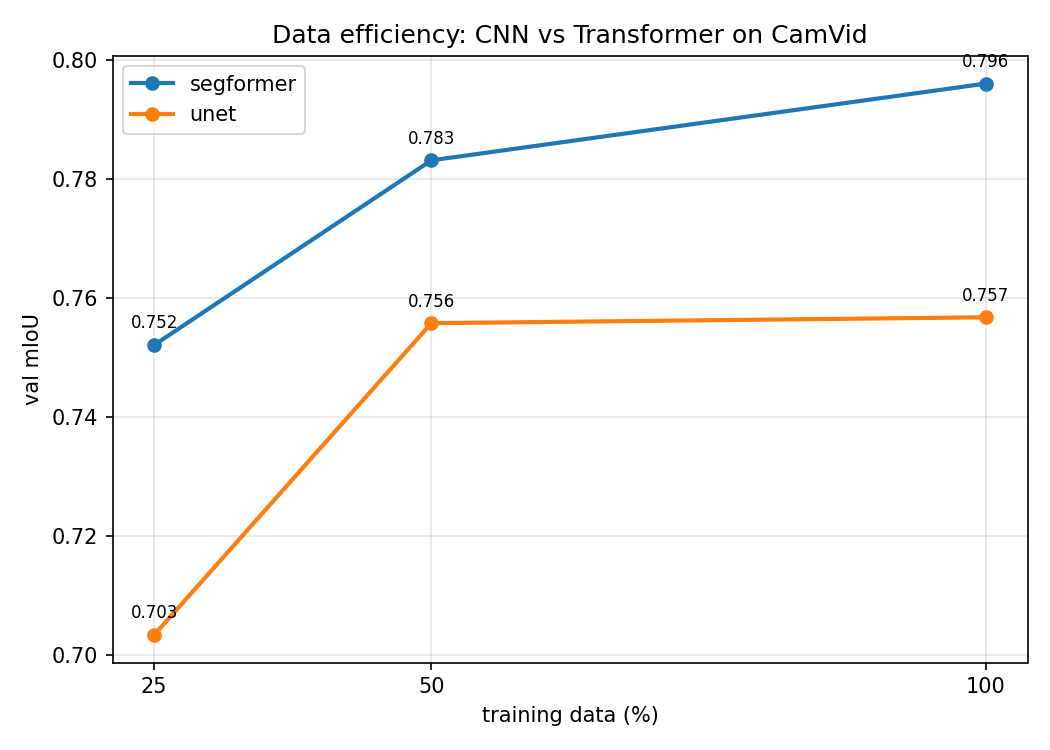
\includegraphics[width=0.8\linewidth]{figures/data_efficiency.png}
    \caption{Data efficiency. SegFormer dominates U-Net at every training-set
    size and, at 25\% data, nearly matches U-Net trained on 100\%.}
    \label{fig:dataeff}
\end{figure}

\subsection{Robustness to Corruptions}

Figure~\ref{fig:robust} reports mIoU under increasing corruption severity.
Averaged over the four corruptions, SegFormer retains 66.5\% of its clean mIoU
at maximum severity versus 54.3\% for U-Net. The aggregate hides a strongly
uneven pattern. Under Gaussian noise U-Net collapses from $0.76$ to roughly
$0.05$, while SegFormer remains functional at $\sim$0.24 --- consistent with
convolution's local sensitivity to pixel-level noise and attention's global
averaging. Motion blur yields a consistent moderate advantage. For fog and
brightness, which apply global photometric shifts that both models effectively
saw through augmentation, the two are close. The architectural advantage
therefore appears specifically when the corruption disrupts \emph{local}
structure.

\begin{figure}[H]
    \centering
    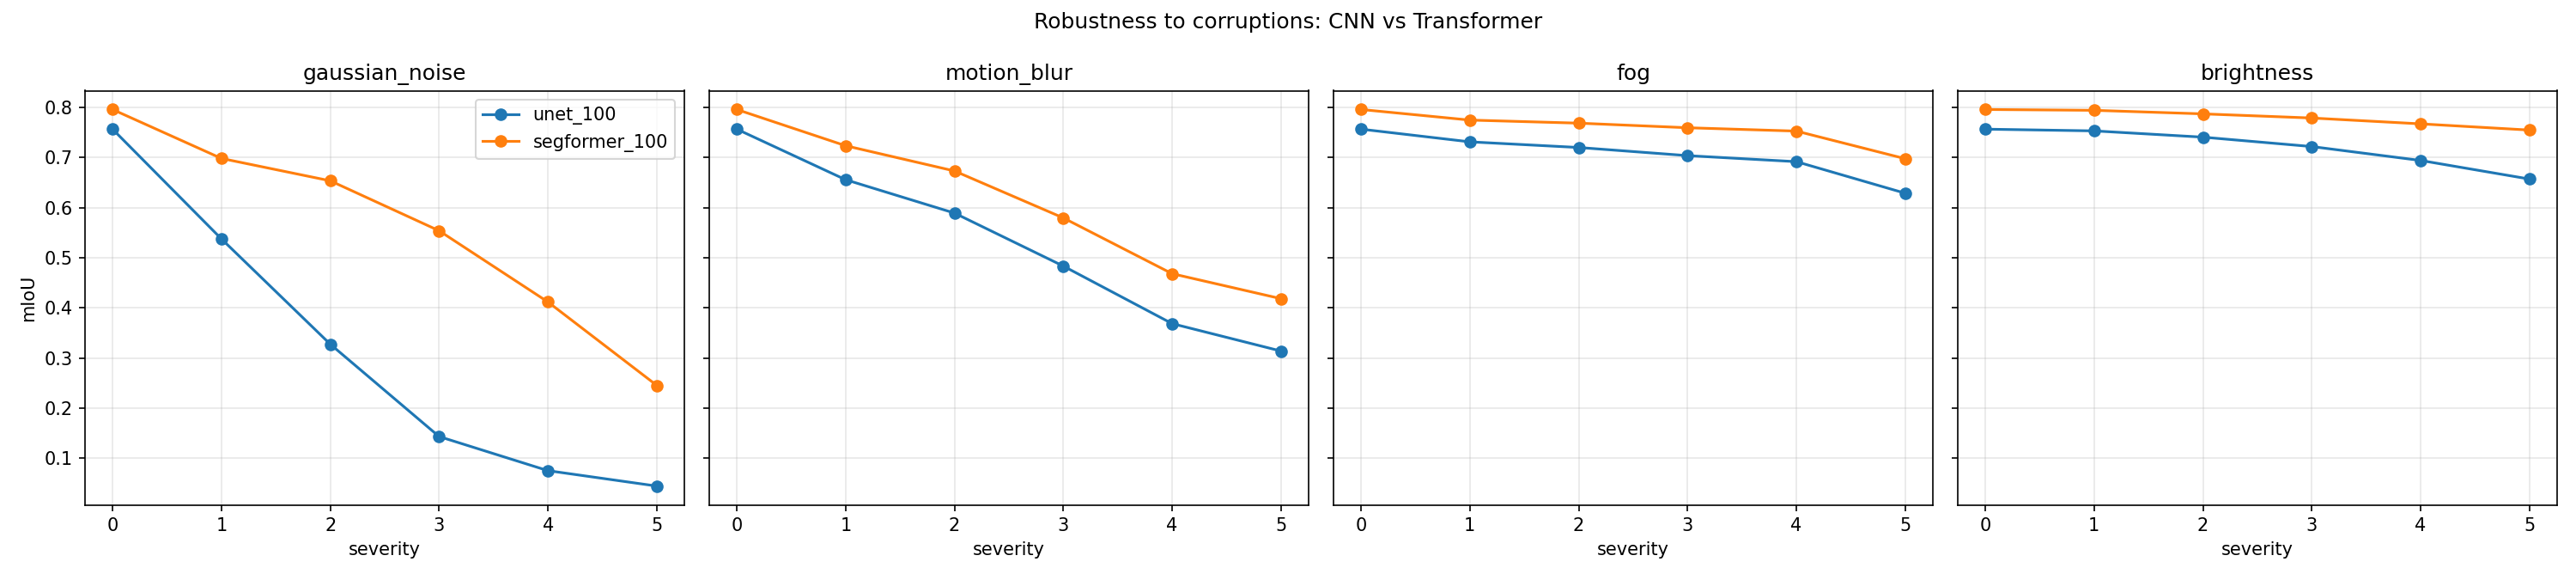
\includegraphics[width=\linewidth]{figures/robustness_val.png}
    \caption{Robustness to test-time corruptions. SegFormer (orange) degrades
    more gracefully than U-Net (blue); the gap is extreme for Gaussian noise
    and negligible for brightness.}
    \label{fig:robust}
\end{figure}

\subsection{Boundary Quality}

Standard IoU is dominated by region interiors and is relatively insensitive to
edge precision. Boundary IoU restricts the computation to a 3-pixel band around
object boundaries. SegFormer produces more accurate boundaries overall
($0.453$ versus $0.416$ mean Boundary IoU, $+0.037$) and leads on 10 of the 11
classes, with the largest gains on thin and irregular classes (\texttt{fence}
$+0.091$, \texttt{tree} $+0.051$, \texttt{pole} $+0.046$). The single exception
is \texttt{sky} ($-0.046$), a large smooth region whose single high-contrast
skyline edge the local convolutional model traces slightly more tightly --- a
reminder that locality is not uniformly inferior.

\subsection{Cross-Dataset Generalization}

To test out-of-distribution generalization, the CamVid-trained models are
evaluated, without retraining, on the 500-image Cityscapes validation set --- a
different country, camera, resolution and annotation style. Cityscapes labels
are mapped onto the 11 CamVid classes; because the mapping is approximate, the
relative gap and retention, not absolute mIoU, are the meaningful quantities,
and both models use the identical mapping.

The result (Table~\ref{tab:cross}) is the most pronounced in the study: the
$+0.039$ in-domain mIoU gap widens to $+0.128$ under domain shift. SegFormer
retains 75\% of its CamVid mIoU ($0.796\!\to\!0.598$) versus 62\% for U-Net
($0.757\!\to\!0.470$). The per-class pattern mirrors the in-domain and
robustness findings: U-Net collapses hardest on the thin and context-dependent
classes, exactly where global context is most valuable.
Figure~\ref{fig:cross} shows representative predictions.

\begin{table}[H]
\centering
\begin{tabular}{lccc}
\toprule
Model & CamVid mIoU & Cityscapes mIoU & Retention \\
\midrule
U-Net     & 0.757 & 0.470 & 62\% \\
SegFormer & 0.796 & \textbf{0.598} & \textbf{75\%} \\
\midrule
$\Delta$  & $+0.039$ & $\mathbf{+0.128}$ & --- \\
\bottomrule
\end{tabular}
\caption{Cross-dataset generalization: CamVid-trained models evaluated
zero-shot on Cityscapes validation (labels remapped).}
\label{tab:cross}
\end{table}

\begin{figure}[H]
    \centering
    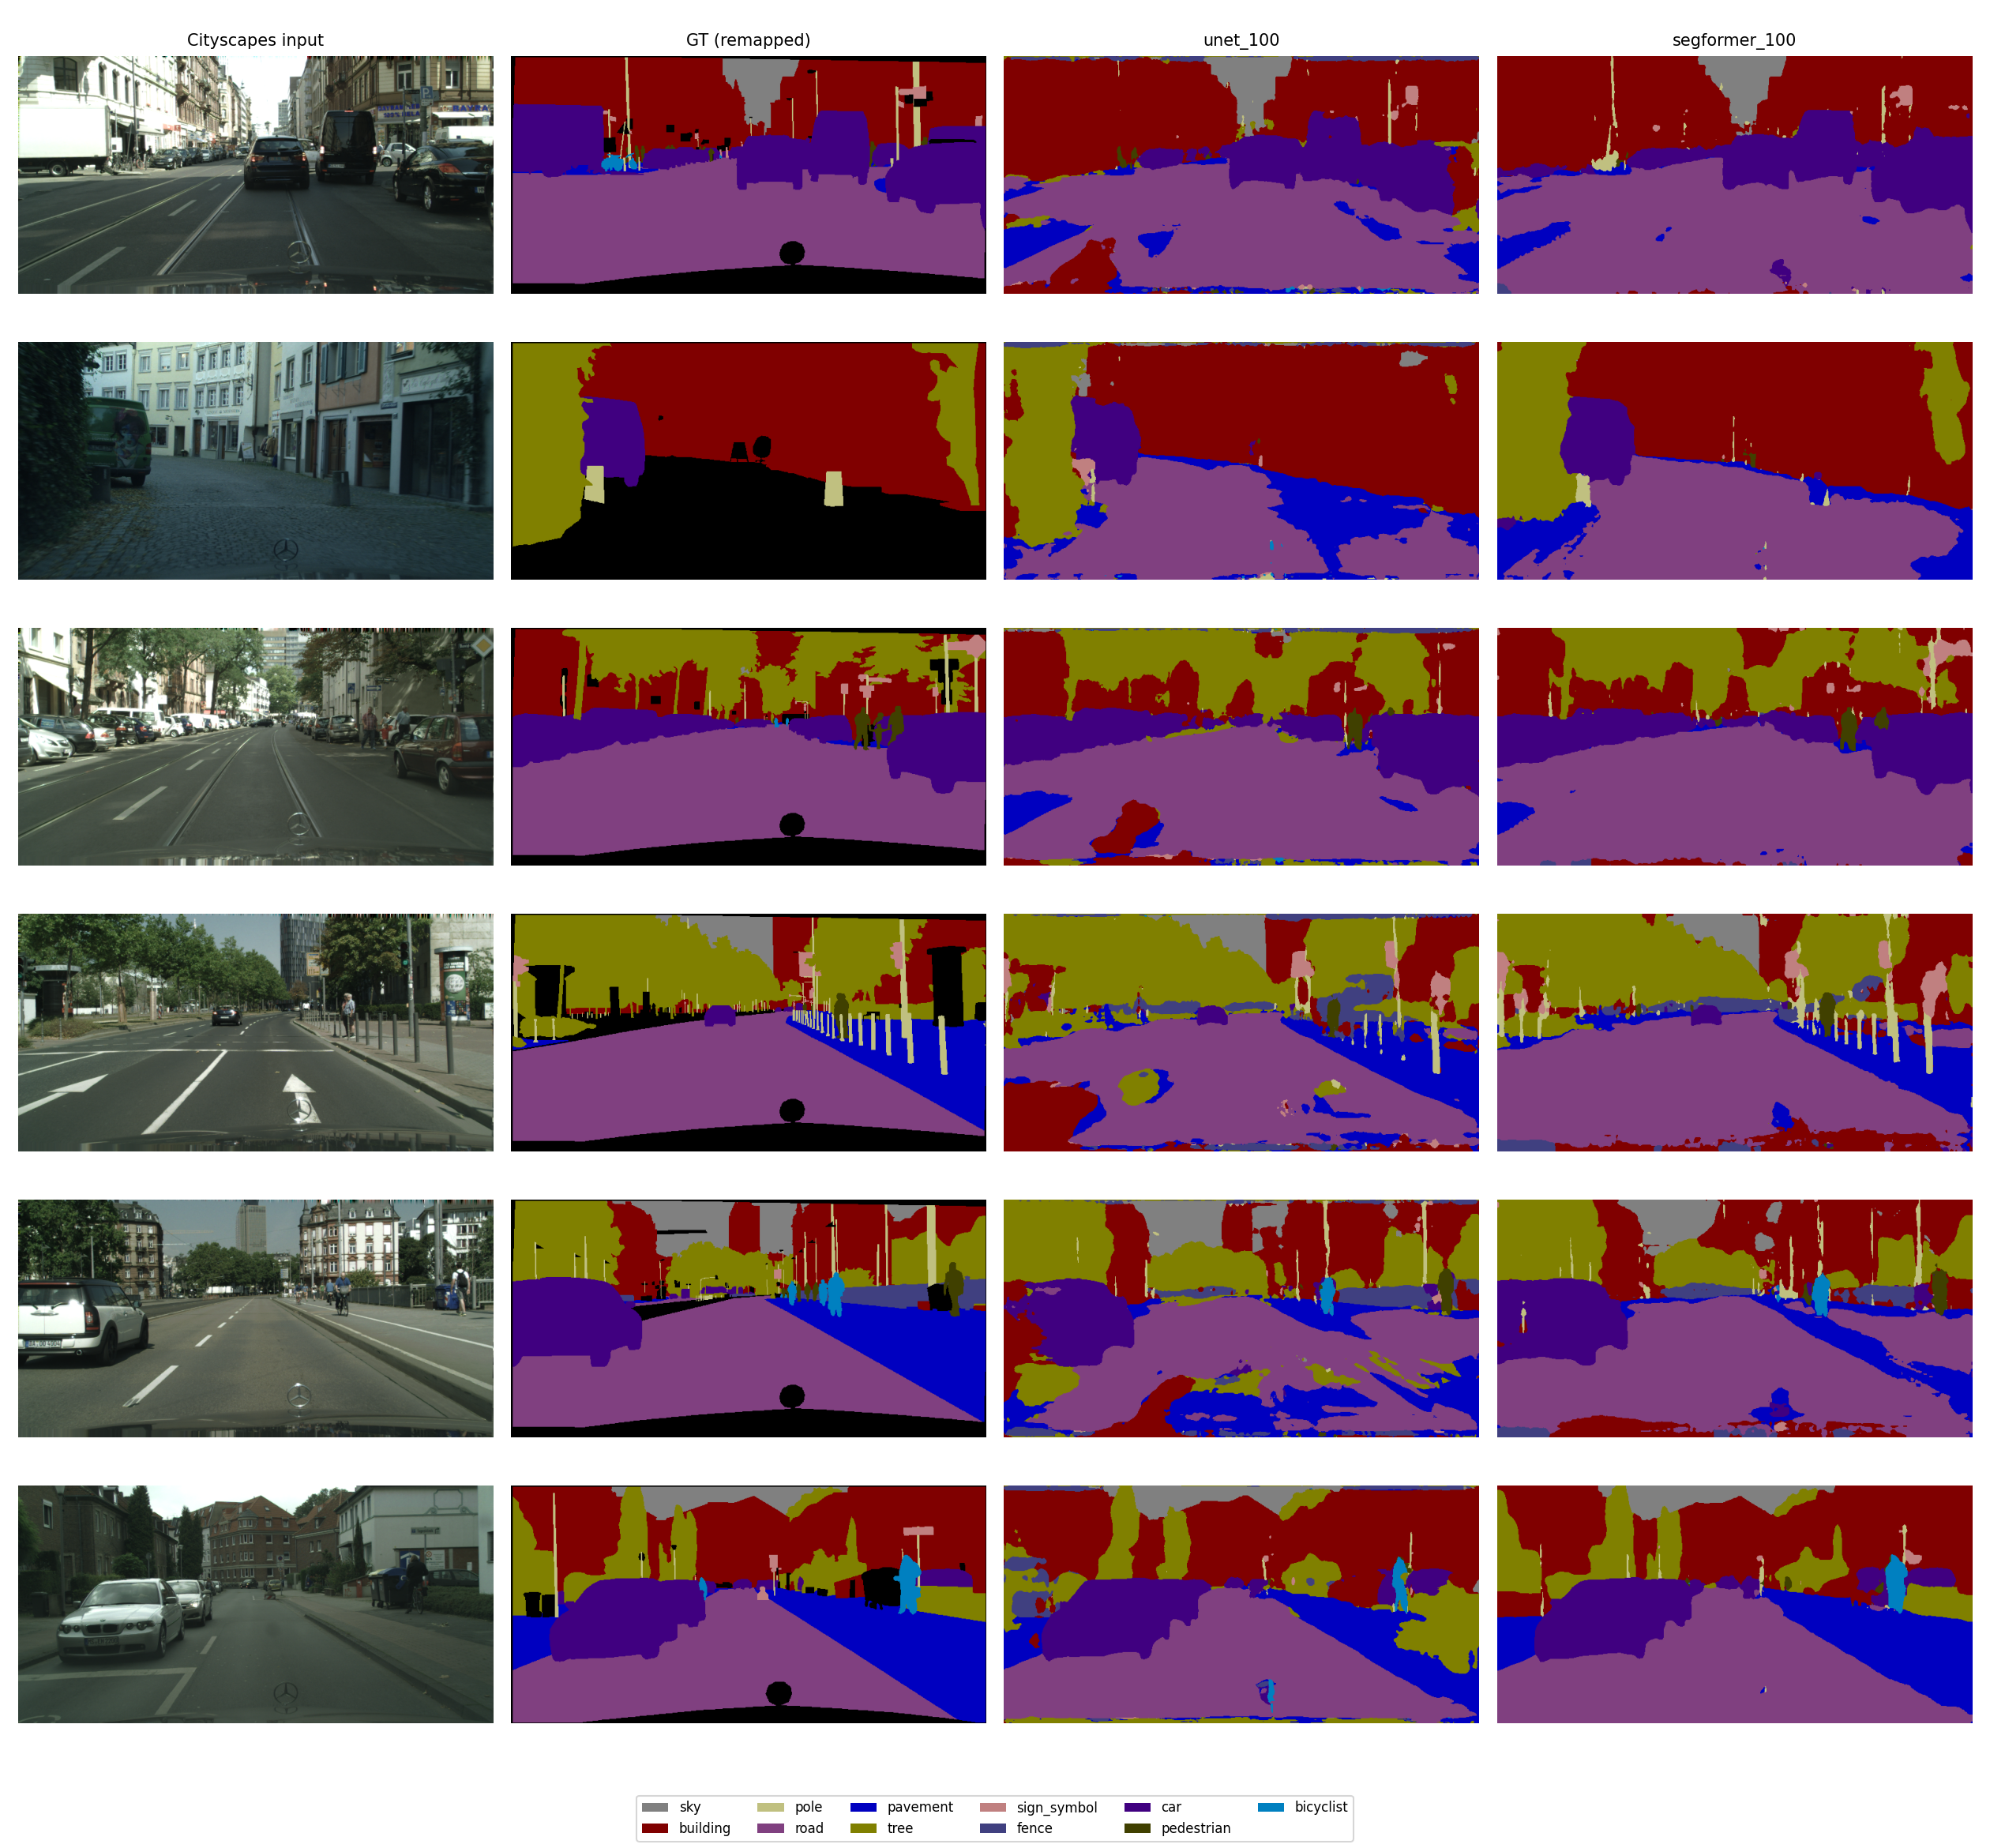
\includegraphics[width=\linewidth]{figures/cityscapes_qualitative.png}
    \caption{Zero-shot predictions on Cityscapes (CamVid-trained models).
    U-Net's predictions fragment on the unfamiliar domain while SegFormer
    remains comparatively coherent.}
    \label{fig:cross}
\end{figure}

\subsection{Test-Time Augmentation}

To confirm the advantage is not an artifact of a single inference setting,
horizontal-flip and multi-scale test-time augmentation (TTA) is applied
identically to both models. Both improve and the gap is essentially unchanged:
SegFormer reaches its best mIoU of $0.808$ with flip+multi-scale TTA versus
U-Net's $0.771$. Evaluating at a higher resolution than training
($736\times960$ versus $384\times480$) \emph{reduced} mIoU for both models, a
train/test resolution-mismatch effect; notably, SegFormer's thin-class accuracy
still improved with extra resolution while U-Net's degraded, again consistent
with the two inductive biases.

\subsection{Qualitative Comparison}

Figure~\ref{fig:qual} compares predictions on the frames where the two models
disagree most. SegFormer produces spatially cleaner masks with fewer speckled
misclassifications on road and pavement, and recovers thin vertical structures
(poles, signs) more continuously, visually corroborating the quantitative
results.

\begin{figure}[H]
    \centering
    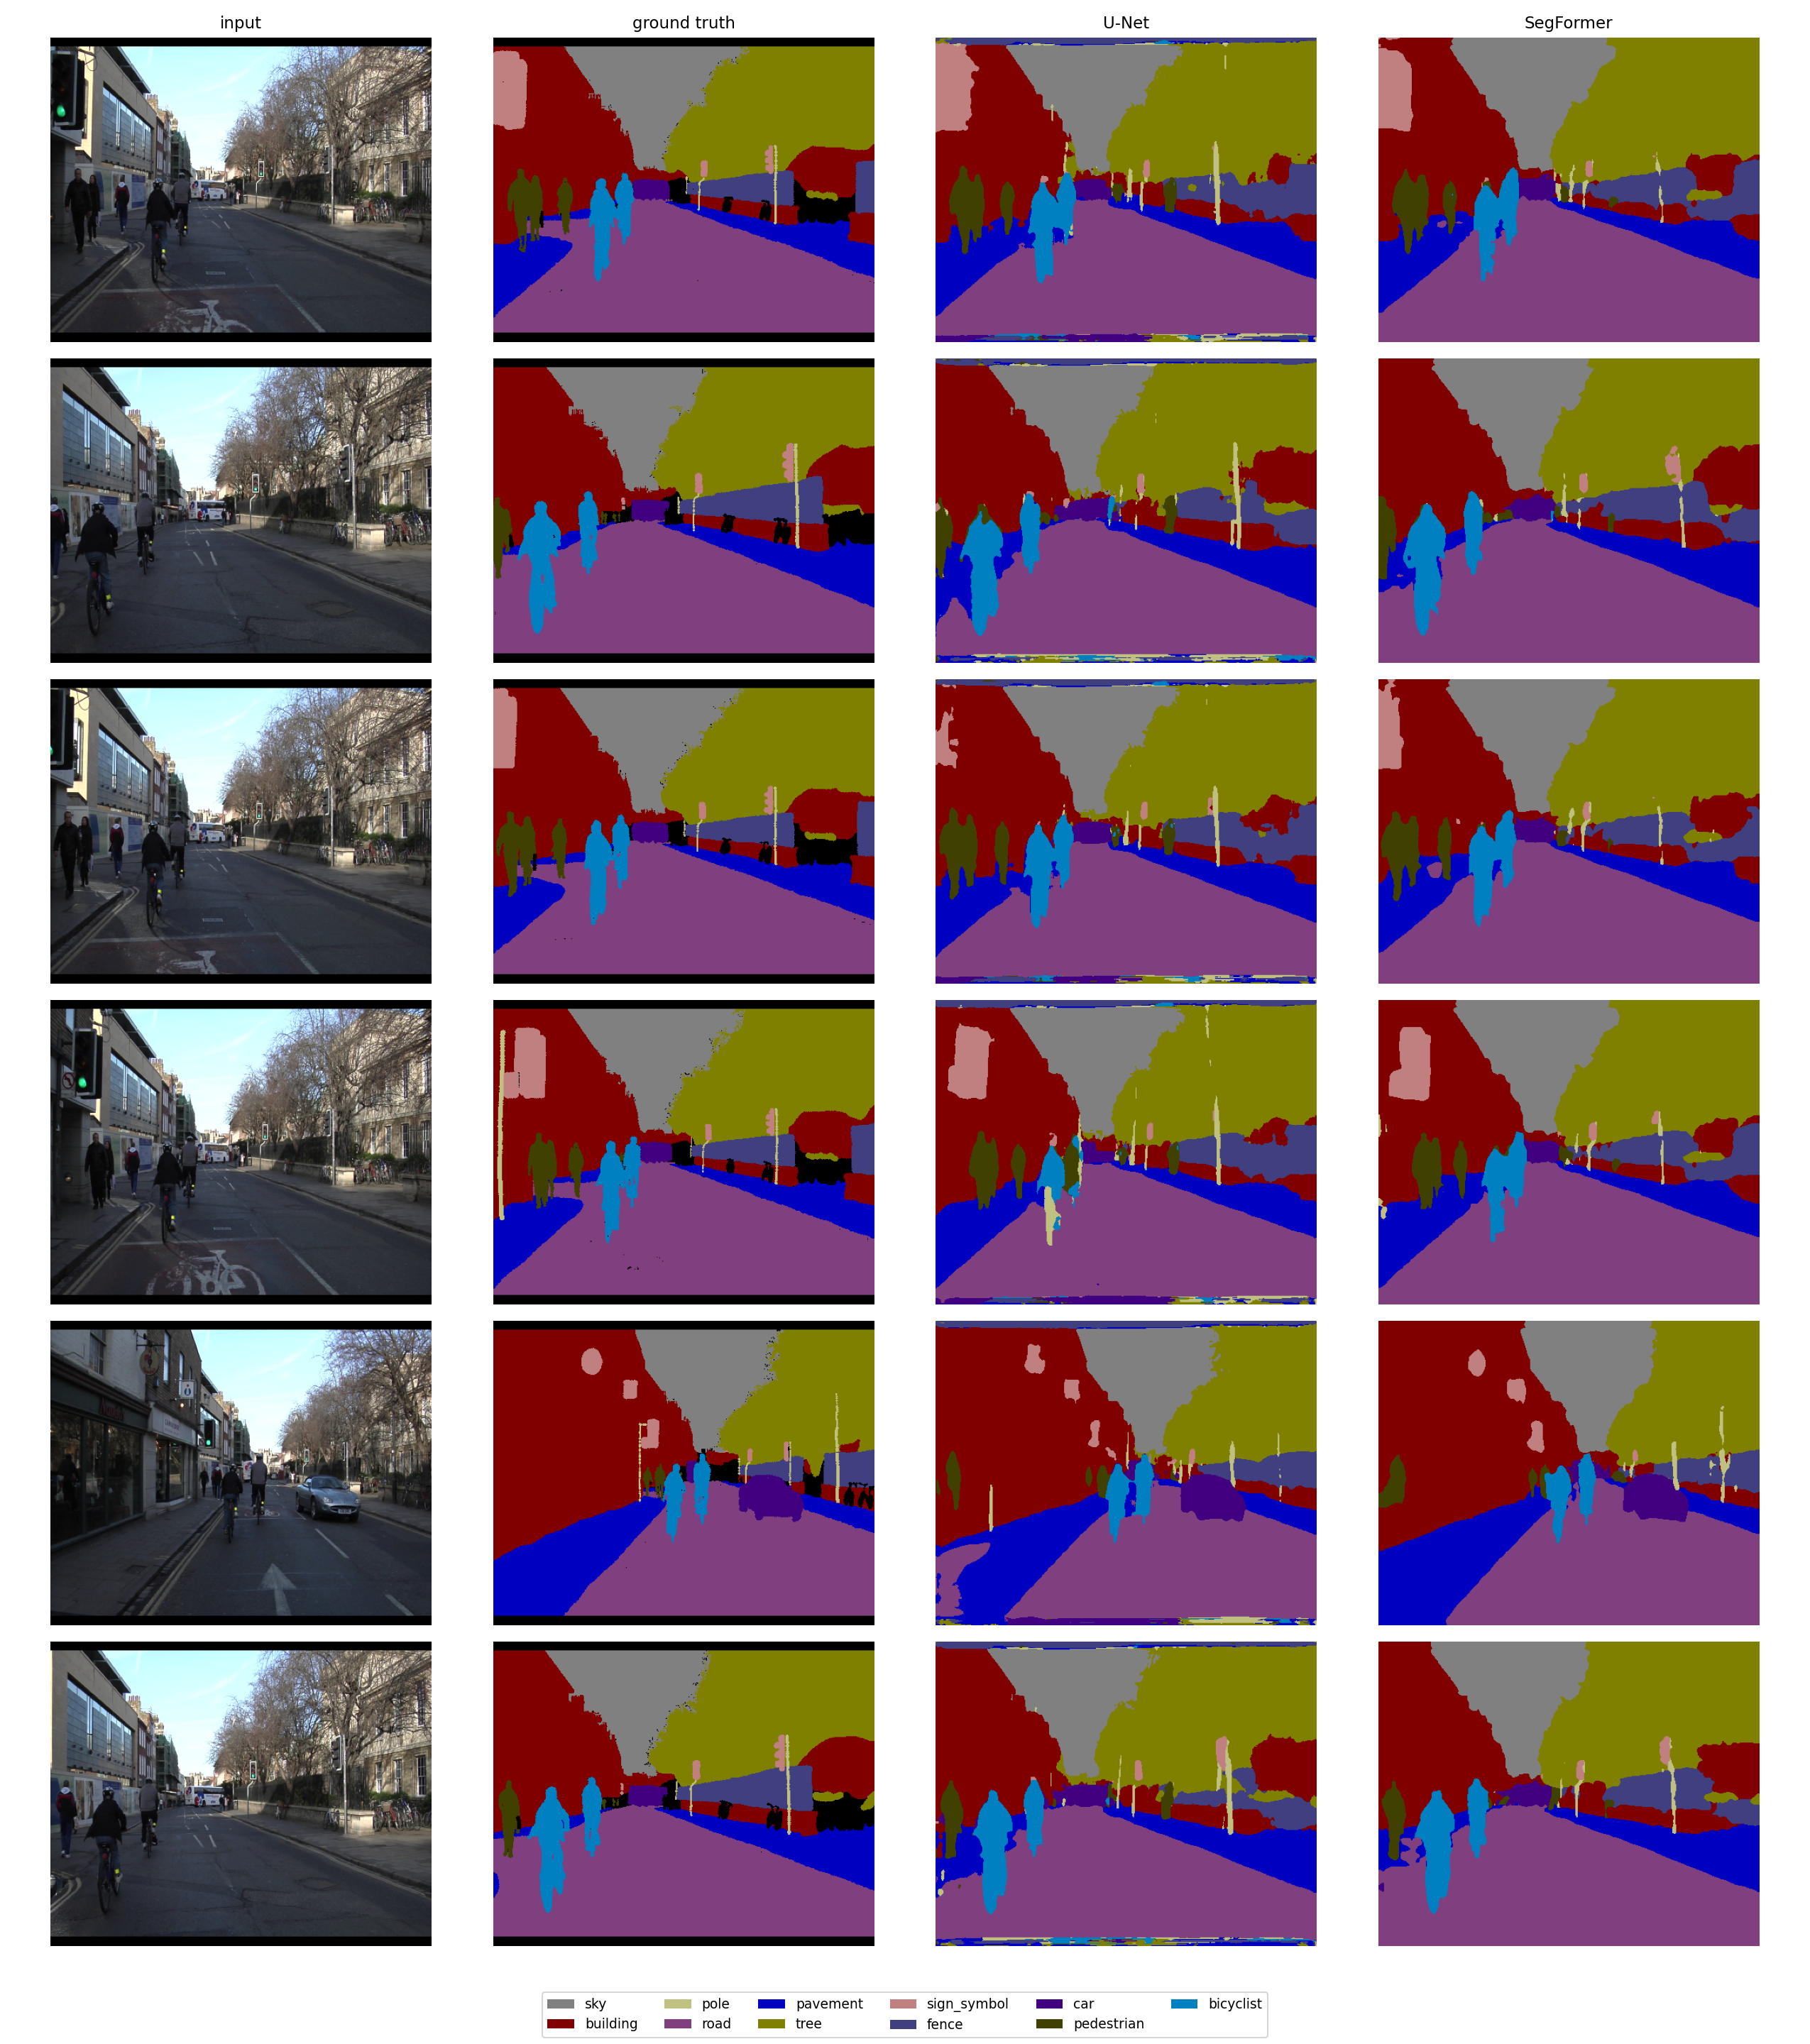
\includegraphics[width=\linewidth]{figures/compare_disagree_val.png}
    \caption{Input, ground truth, U-Net and SegFormer on the most-disagreeing
    validation frames.}
    \label{fig:qual}
\end{figure}

% ----------------------------- Discussion ----------------------------------
\section{Discussion and Limitations}

Across all axes a single theme recurs, and it strengthens monotonically: the
transformer's advantage grows with the difficulty of the condition. It is
marginal on large in-domain classes ($+0.04$ mIoU overall), larger on thin and
context-dependent classes, larger still under input corruption ($66.5\%$ versus
$54.3\%$ retained), and largest under domain shift to Cityscapes ($+0.128$
mIoU, three times the in-domain gap). The harder the setting departs from the
easy, in-distribution, large-object regime, the more global self-attention
outperforms local convolution.

Several limitations temper these conclusions. The comparison uses a single
small dataset, and the held-out evaluation is on the validation set in the
standard course setting. One representative per family is compared rather than a
sweep of architectures, and both rely on ImageNet pretraining, so this is a
fine-tuning rather than a from-scratch comparison --- indeed the data-efficiency
result is partly a statement about pretrained features. The cross-dataset label
mapping is approximate, so the Cityscapes numbers are indicative rather than
exact. Finally, the contrast is not a mathematically pure ablation: SegFormer's
Mix-FFN contains $3\times3$ convolutions and its decoder is lighter than
U-Net's, so the comparison is between an attention-dominated model and a
convolution-only one rather than attention versus convolution in isolation.

% ----------------------------- Conclusion ----------------------------------
\section{Conclusion}

This project presented a controlled, parameter-matched, identically-trained
comparison of a convolutional (U-Net) and a transformer-based (SegFormer) model
for semantic segmentation on CamVid. SegFormer outperformed U-Net in accuracy
($+0.033$ mIoU, significant over three seeds), data efficiency (matching
full-data U-Net with 25\% of the data), robustness (66.5\% versus 54.3\% mIoU
retained under corruption), boundary quality ($+0.037$ mean Boundary IoU), and
cross-dataset generalization to Cityscapes ($+0.128$ mIoU). In every case the
margin scaled with the need for global context, providing a concrete,
multi-axis illustration of how the inductive biases of convolution and
self-attention manifest in semantic segmentation. Future work could extend the
comparison to additional datasets, train from scratch to separate the effect of
pretraining, and include a wider range of architectures.

% ----------------------------- References ----------------------------------
\section*{References}

\begin{itemize}
  \item U-Net: O. Ronneberger, P. Fischer, T. Brox, ``U-Net: Convolutional
  Networks for Biomedical Image Segmentation,'' MICCAI, 2015.
  \item SegFormer: E. Xie et al., ``SegFormer: Simple and Efficient Design for
  Semantic Segmentation with Transformers,'' NeurIPS, 2021.
  \item DeepLab: L.-C. Chen et al., ``DeepLab: Semantic Image Segmentation
  with Deep Convolutional Nets, Atrous Convolution, and Fully Connected CRFs,''
  IEEE TPAMI, 2018.
  \item Vision Transformer: A. Dosovitskiy et al., ``An Image is Worth
  16x16 Words: Transformers for Image Recognition at Scale,'' ICLR, 2021.
  \item Boundary IoU: B. Cheng et al., ``Boundary IoU: Improving Object-Centric
  Image Segmentation Evaluation,'' CVPR, 2021.
  \item Cityscapes: M. Cordts et al., ``The Cityscapes Dataset for Semantic
  Urban Scene Understanding,'' CVPR, 2016.
  \item CamVid: G. J. Brostow et al., ``Semantic Object Classes in Video:
  A High-Definition Ground Truth Database,'' Pattern Recognition Letters, 2009.
  \item segmentation-models-pytorch: \url{https://github.com/qubvel/segmentation_models.pytorch}
  \item HuggingFace Transformers: \url{https://github.com/huggingface/transformers}
\end{itemize}

\end{document}
